\section{Deterministic PDA and languages}

Nondeterminism is absent if the transition function $\delta$ is one-valued and if $\delta (q, a, A)$ is defined then $\delta(q, \varepsilon, A)$ is undefined and 
if $\delta(q, \varepsilon, A)$ is defined then $\delta (q, a, A)$ is undefined for every $a \in \Sigma$. If the transition function does not exhibit any form of 
non-determinism, then the automaton is deterministic and the recognized language is deterministic, too. 

The family DET of the deterministic free languages is strictly contained in the family CF of all the free languages. 

If we denote by $L$, $D$ and $R$ a language that belongs to the family CF, DET, and REG we have the following closure properties: 
\begin{figure}[H]
    \centering
    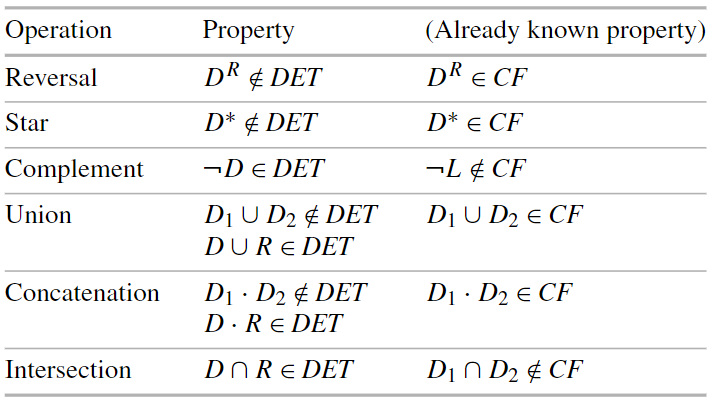
\includegraphics[width=0.8\linewidth]{images/PDAclosure.png}
\end{figure}